\documentclass{article}
\usepackage[submission]{colm2026_conference}
\usepackage{microtype}
\usepackage{hyperref}
\usepackage{url}
\usepackage{booktabs}
\usepackage{lineno}
\usepackage{graphicx}
\usepackage{wrapfig}
\usepackage{amsmath}
\usepackage{xcolor}
\definecolor{darkblue}{rgb}{0,0,0.5}
\hypersetup{colorlinks=true, citecolor=darkblue, linkcolor=darkblue, urlcolor=darkblue}

\title{Low-Cost Geometric Directions in Frozen Speech Models:\\
Where a Training-Free Deepfake-Hardness Signal Helps---and Where It Does Not}

\author{Anonymous authors\\Paper under double-blind review}

\begin{document}
\linenumbers
\maketitle

\begin{abstract}
Deepfake-speech detectors are inconsistent in two systematic ways: against a
fixed detector some synthesis systems evade detection far more often than others,
and a detector trained on one recording domain often fails on another. Working
entirely at small scale---one GPU, a frozen $\sim$100M-parameter encoder, and no
detector retraining---we show that much of this inconsistency is legible in the
\emph{geometry} of the frozen representation. Inside the frozen encoder there is a
single natural-versus-synthetic direction, and how far a synthesis system's
utterances \emph{spread} along it predicts how hard that system is to detect---the
only quantity, out of 83 we tested, to survive a global false-discovery-rate
correction. Two further results follow. First, the direction is not universal: it
rotates across datasets to near-orthogonality (and reverses sign), the geometric
reason detectors fail to transfer. Second, it is a training-free corrective signal
whose value is conditional on headroom: it reduces a weak detector's error by
$\approx$21\% while yielding no measurable change for an already-strong one. Every
quantitative claim is independently audited, with confirmed and exploratory results
separated. The contribution is a precise account of where low-cost geometric
directions in frozen models help---and where they do not.
\end{abstract}

\section{Introduction}
Synthetic speech is now realistic enough that its detection is a security
necessity, and the standard defence is a classifier that flags synthetic
utterances. Yet detectors are unreliable in two ways that aggregate accuracy
hides: against a fixed detector some synthesis systems evade far more often than
others, and a detector tuned on one recording domain often fails on another.
Neither had a clean explanation.

We provide one, and we obtain it at small scale. Modern detectors sit on top of a
large frozen self-supervised (SSL) speech encoder \citep{chen2022wavlm}; we treat
that frozen representation as the object of study, before any decision boundary is
drawn. Our central finding is a \textbf{natural-versus-synthetic axis}: a single
direction running from natural to synthetic speech. A system whose utterances
cluster tightly along this axis is detected easily; one whose utterances spread
along it is hard. That spread, $\mathrm{sd}_{\mathrm{along}}$, is our predictor.

Three results follow, each established at small scale. (i)~\emph{The law:}
$\mathrm{sd}_{\mathrm{along}}$ predicts per-system hardness and is the single
quantity, among 83 tested, to survive global multiple-testing correction
(Sec.~\ref{sec:law}). (ii)~\emph{The axis rotates:} each dataset has its own axis
pointing a different way, so a transferred axis is uninformative---the geometric
reason transfer fails (Sec.~\ref{sec:rotate}). (iii)~\emph{A training-free
corrective signal, conditioned on headroom:} fusing the axis into a detector's
score requires no retraining and no labels and improves detection, but only when
the detector has headroom (Sec.~\ref{sec:lever}). We hold a high evidential bar
throughout: an independent audit recomputed every number and is reported in-line
(Sec.~\ref{sec:audit}).

\begin{wrapfigure}{r}{0.44\linewidth}
\centering
\vspace{-8pt}
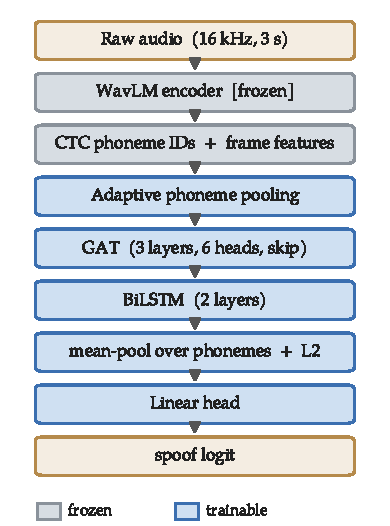
\includegraphics[width=\linewidth]{figs/fig1_architecture.pdf}
\vspace{-14pt}
\caption{The WavLM-GAT detector, redrawn; architecture after
\citet{zhang2025phoneme}. A frozen WavLM encoder yields phoneme IDs and features; a
small trainable head (adaptive phoneme pooling, GAT, BiLSTM, linear) emits a spoof
logit. All our geometry is measured in the frozen layer-12 space.}
\label{fig:arch}
\vspace{-8pt}
\end{wrapfigure}

\section{Setup}
\textbf{Detector.} Our primary detector (WavLM-GAT) is the phoneme-level
graph-attention model of \citet{zhang2025phoneme}: a frozen WavLM encoder feeds
adaptive phoneme pooling, a 3-layer 6-head graph-attention network
\citep{velickovic2018graph} with skip connections, a BiLSTM, and a linear head
(Fig.~\ref{fig:arch}). The encoder is frozen ($\sim$95M parameters); only the
$\sim$13M-parameter head trains. For architecture generality we also use AASIST
\citep{jung2022aasist}.

\textbf{Corpora and hardness.} The hardness law is established on MLAAD
\citep{muller2024mlaad} (61 text-to-speech systems with $\geq 8$ utterances). The
training-free lever and the axis-rotation check additionally use ASVspoof~2019~LA
\citep{wang2020asvspoof}. Per-system hardness is $1-\mathrm{AUC}$ of the detector's
scores for that system against a shared bona-fide pool; on a held-out check the
metric has split-half reliability $0.76$ ($R^2$ ceiling $\approx 0.86$).

\textbf{Axis.} Per corpus we estimate a natural-versus-synthetic direction $w$ in
mean-pooled frozen WavLM-L12 space as the (unsupervised) bona-fide$-$synthetic
centroid difference, leave-one-system-out so a held-out system never informs its
own axis. For each system we record $\mathrm{sd}_{\mathrm{along}}$, the standard
deviation of its per-utterance projections onto $w$.

\textbf{Compute.} Everything runs on a single GPU; the largest single training run
is $\approx 10^{16}$ FLOPs (well under a $10^{20}$ budget), and all geometry re-runs
from cached embeddings in minutes.

\section{A Natural--Synthetic Axis Predicts Detection Hardness}
\label{sec:law}
Across 61 MLAAD systems, per-system hardness rises with
$\mathrm{sd}_{\mathrm{along}}$ (Fig.~\ref{fig:results}a; Spearman $\rho=0.60$,
$p<10^{-6}$; leave-one-system-out $R^2=0.277$, permutation $p=2.5\times10^{-4}$;
bootstrap $\rho$ CI $[0.41,0.73]$). A system whose utterances straddle the
boundary---some appearing essentially genuine to the encoder---is difficult to
detect, and those near-genuine utterances are the ones that evade.

This is the most robust predictor we identified. Of \textbf{83} quantities tested
across the study, $\mathrm{sd}_{\mathrm{along}}$ is the \emph{only} one to survive
a global Benjamini--Hochberg correction. It survives leave-one-system jackknifing
($\rho$ range $0.58$--$0.63$) and strengthens as measurement
noise falls: $\rho=0.60\!\to\!0.64\!\to\!0.69$ at $\geq 8/12/16$ utterances per
system---the attenuation signature of a real effect. Against the $0.86$
reliability ceiling it captures $\approx$32\% of the \emph{explainable} hardness
variance: a partial but robust account.

\textbf{Directionality, not circularity.} Because a centroid axis can resemble a
detector's own logit direction, we verified that the mechanism is directional,
not an artifact of magnitude. Substituting the top discriminative directions of the
representation with class-blind values degrades detection
($\Delta\mathrm{AUC}=-0.032$), whereas the identical operation on the
equal-magnitude orthogonal residual does not ($+0.004$); the contrast is
consistent across all three seeds (we do not claim significance at $n=3$). An earlier ungated version of this intervention inflated a spurious ``compactness''
effect by $\approx$80\%; closing that leak isolates the directional mechanism. Finally, the rank-order law
\emph{replicates on a different architecture}: on AASIST fine-tuned on MLAAD,
$\mathrm{sd}_{\mathrm{along}}$ still ranks hardness ($\rho=+0.35$, $p=0.006$). We
are precise that only the rank-order form transfers---the $R^2$ regression form
does not on AASIST ($r^2\approx0$)---and report both.

\begin{figure}[t]
\centering
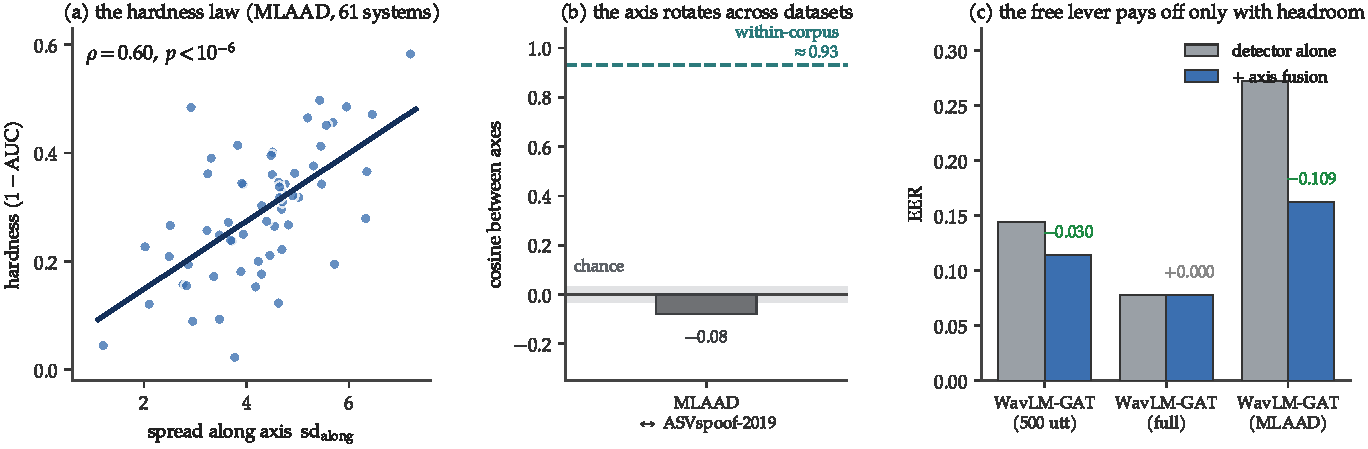
\includegraphics[width=\linewidth]{figs/fig2_results.pdf}
\caption{\textbf{(a)}~Spread along the corpus-internal natural--synthetic axis
predicts MLAAD hardness across 61 systems. \textbf{(b)}~The axis rotates: the
MLAAD and ASVspoof-2019 internal axes are near-orthogonal and slightly negative
($\cos\approx-0.08$), far below within-corpus reliability ($\approx0.93$, dashed)
and inside the high-dimensional chance band ($\approx\!0.03$, grey).
\textbf{(c)}~Training-free axis fusion reduces a weak WavLM-GAT's error
($\Delta$EER $-0.030$, and $-0.11$ for an under-trained MLAAD detector) but yields
no change for an already-strong one ($+0.000$).}
\label{fig:results}
\end{figure}

\section{The Axis Rotates Across Datasets}
\label{sec:rotate}
Why does a predictor (or detector) fit on one corpus fail on another? Because the
direction it relies on is not the same direction elsewhere. Each corpus's internal
axis is estimated almost noiselessly (split-half cosine $\approx0.93$), yet the
axis learned on MLAAD and the axis learned on ASVspoof-2019 are
near-orthogonal---and in fact slightly negative ($\cos\approx-0.08$;
Fig.~\ref{fig:results}b), against a $768$-dimensional chance floor of
$\approx0.03$. A transferred axis therefore points, if anything, the wrong way. The
operational lesson is direct: an axis-based hardness diagnostic must be
re-estimated on the target recording domain, and a detector's per-system error
profile from one corpus should not be trusted on another. We cannot fully exclude
that part of the rotation reflects recording-channel nuisance rather than
synthesis semantics; either way the lesson is unchanged.

\section{Training-Free Axis Fusion Helps Only Under Detector Headroom}
\label{sec:lever}
Because the axis identifies \emph{which} systems a detector will struggle with,
its projection can be fused into the detector's decision,
$z(\mathrm{logit})+\lambda\,z(\mathrm{axis})$, with no retraining and no new
labels. Whether this helps depends entirely on headroom
(Fig.~\ref{fig:results}c). We trained a deliberately weak WavLM-GAT on only 500
utterances; the unsupervised axis reduced its equal-error rate from $0.144$ to
$0.114$ ($\Delta$EER $=-0.030$, 95\% CI $[-0.046,-0.013]$, $p\approx0$), improving
all five attack-disjoint folds---a $\approx$21\% relative reduction. The
\emph{identical} procedure applied to a strong, near-ceiling WavLM-GAT (EER
$0.078$) produced no change distinguishable from noise ($\Delta$EER $=-0.0004$ to
$+0.004$, $p\approx0.56$--$0.80$). In domain on MLAAD, where the base detector is
likewise far from ceiling, the same zero-training centroid fusion improves EER from
$0.272$ to $0.163$ (axis alone $0.187$), negative across all folds and seeds. Axis
fusion therefore provides a practical, training-free improvement precisely when the
base detector is undertrained, and none when it is already strong; in both cases the
deployed detector is left untouched.

\section{Independent Audit of the Reported Claims}
\label{sec:audit}
Every quantitative claim was checked by an independent audit that recomputed each
number from cached artifacts, returning a tally of 8 verified, 6 mislabeled, 5
misleading, and 2 contradicted claims; each was corrected or removed. The
corrections are substantive, not cosmetic: a cross-corpus cosine reported as
$+0.36$ was in fact negative (the axis rotates with the \emph{wrong} sign); an
$R^2$ of $0.316$ attributed to $\mathrm{sd}_{\mathrm{along}}$ was in fact a
three-feature triplet model, the correct single-feature value being $0.277$; a
``small residual causal effect'' disagreed in sign across seeds and was dropped;
and ``13 interventions'' was corrected to the 22 conditions actually run. We report
the audit in-line and separate confirmed from exploratory claims throughout.

\section{Limitations and Conclusion}
The law is a text-to-speech phenomenon: on voice-conversion attacks all predictors
give $\rho\approx0$, consistent with converted speech inheriting its content from
source speech. All geometry uses a single SSL backbone (WavLM); generality to
wav2vec\,2.0 or HuBERT is untested. The law rests on $n=61$ systems and the causal
contrasts on only three seeds, so the directional mechanism is trustworthy in sign
but not powered as a significance claim. Cross-dataset \emph{prospective}
prediction of hardness---using one corpus's axis to rank a never-seen corpus's
systems in advance---remains unconfirmed and is left as future work. Within these
bounds, the contribution is a reusable finding for small-scale research: a
low-cost, frozen, training-free geometric direction is a genuine tool for
understanding and partially correcting deepfake detectors, and we have delimited
precisely where it applies (weak detectors, within a dataset) and where it does not
(across datasets, or on already-strong detectors).

\subsubsection*{Reproducibility statement}
All results come from a single-GPU pipeline with a frozen $\sim$95M-parameter
encoder and a $\sim$13M-parameter trainable head ($\ll 3$B parameters); the largest
single training run is $\approx 10^{16}$ FLOPs. We report estimated FLOP budgets and
release logs, checkpoints, cached embeddings, and the full audit, with scripts that
regenerate every reported number.

\bibliography{references}
\bibliographystyle{colm2026_conference}

\end{document}
